Note: typos and spelling errors have been corrected, and spelling has been changed from UK standard to US standard in some cases, but no other changes have been made to the attendee responses.

\hspace{0.2cm}

\noindent \textbf{1. Please indicate how strongly you agree or disagree with the following statements}

\begin{table}[h!]
\centering
\caption{General questions about the conference program}
\label{tab:survey_program}
{\scriptsize
\begin{tabular}{@{}lcccccc@{}}
\toprule
\multirow{2}{*}{Question} & strongly & somewhat & agree & somewhat & strongly &
\multirow{2}{*}{Total} \\
& disagree & disagree & & agree & agree & \\
\midrule
\rowcolor{lightgray} The plenary sessions had a good & & & & & & \\
\rowcolor{lightgray} mix of topics and speakers. &
\multirow{-2}{*}{5} &
\multirow{-2}{*}{3} &
\multirow{-2}{*}{8} &
\multirow{-2}{*}{11} &
\multirow{-2}{*}{18} &
\multirow{-2}{*}{45} \\
The balance was right between &
\multirow{2}{*}{6} &
\multirow{2}{*}{2} &
\multirow{2}{*}{7} &
\multirow{2}{*}{9} &
\multirow{2}{*}{21} &
\multirow{2}{*}{45} \\
talks, panels, and lightning talks. & & & & & & \\
\rowcolor{lightgray} There was sufficient time for discussion. &
6 &
6 &
8 &
9 &
16 &
45 \\
\bottomrule
\end{tabular}
}
\end{table}

%Figures have been inserted with little/no formatting.
%Figures are in *.png but can be remade to other formats
%\todo{Place 3 figures in 1 row with Latex}
%\begin{figure}[h!]
%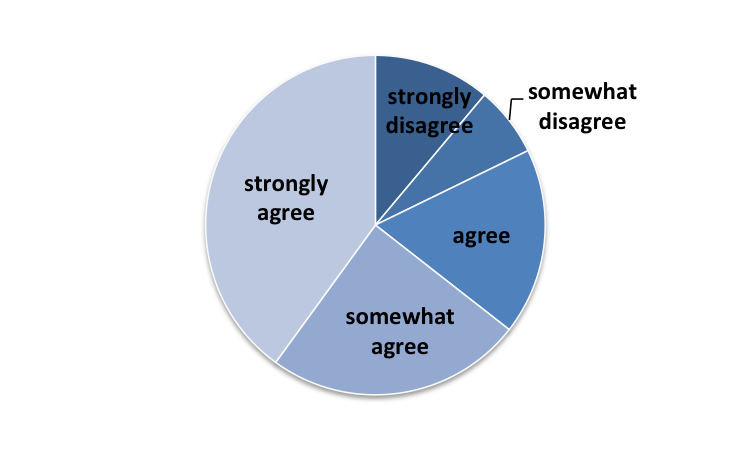
\includegraphics[width=0.3\textwidth]{figures/SurveyFig1rev}
%\caption{The plenary sessions had a good mix of topics and speakers.
%\label{fig:SFig1}}
%\end{figure}
%\begin{figure}[h!]
%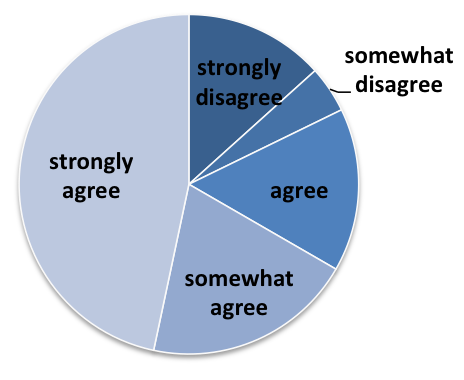
\includegraphics[width=0.3\textwidth]{figures/SurveyFig2rev}
%\caption{The balance was right between talks, panels, and lightning talks.
%\label{fig:SFig2}}
%\end{figure}
%\begin{figure}[h!]
%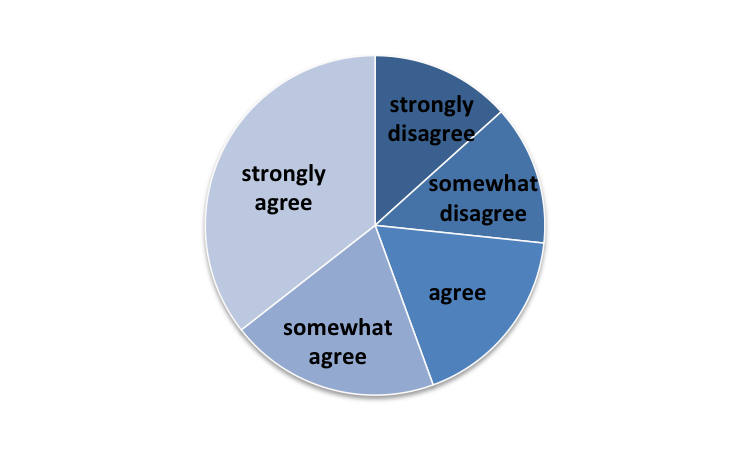
\includegraphics[width=0.3\textwidth]{figures/SurveyFig3rev}
%\caption{There was sufficient time for discussion.
%\label{fig:SFig3}}
%\end{figure}


\begin{figure}[!htb]
    \captionsetup[subfigure]{position=b}
    \centering
    \subcaptionbox{
    The plenary sessions had a good mix of topics and speakers.
    \label{fig:SFig1}
    }{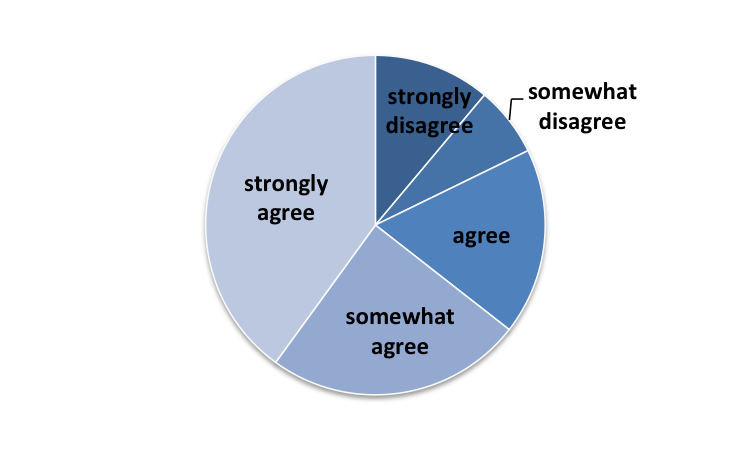
\includegraphics[width=.33\linewidth]{figures/SurveyFig1rev}}
    ~
    \subcaptionbox{
    The balance was right between talks, panels, and lightning talks.
    \label{fig:SFig2}
    }{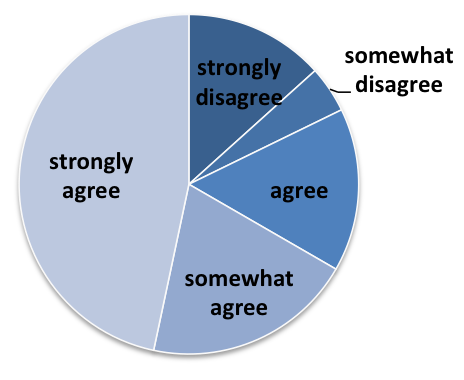
\includegraphics[width=.32\linewidth]{figures/SurveyFig2rev}}
    ~
    \subcaptionbox{
    There was sufficient time for discussion.
    \label{fig:SFig3}
    }{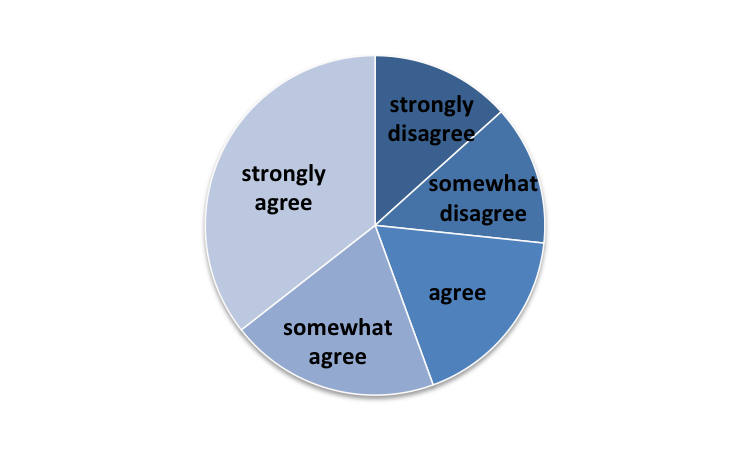
\includegraphics[width=.26\linewidth]{figures/SurveyFig3rev}}
    \caption{Responses to general questions about the conference program}
\end{figure}

\noindent \textbf{2. What part of the meeting was the most valuable? select all that apply}

\begin{figure}[h!]
    \centering
    \begin{tabular}{@{}c@{}}
        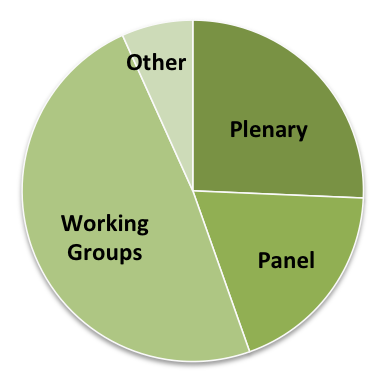
\includegraphics[width=0.35\textwidth]{figures/SurveyFig4rev}%
    \end{tabular}
    \qquad
    \rowcolors{1}{}{lightgray}
    \begin{tabular}{@{}lc@{}}
    \toprule
    Answer & Count \\
    \midrule
    Plenary & 19 \\
    Panel & 14 \\
    Working Groups & 36 \\
    Other & 5 \\
    Total & 74 \\
    \bottomrule
    \end{tabular}
    \caption{Responses to ``What part of the meeting was the most valuable?''}
    \label{fig:SFig4}
\end{figure}

\newpage
\noindent \textbf{3. What additional topics would you like to see discussed at the next meeting?}

\begin{itemize}
\item Concrete reports about best practices
\item considerations of software licensing, build systems, delivery (source vs binary vs whatever) - but of course these are ``later'' issues... first one needs the software to not be hidden, to have version control, have a README, etc.
\item Container sustainability practices
\item education, training interns
\item Explicit follow-up at WSSSPE5 on all the activities that were created at WSSPE4.  These should be at least lightning talks, perhaps with their own session.
\item financial models for sustaining software
\item Frameworks for building software
\item have a short beginning presentation for each working group and a short ending presentation
\item How software development training can be adapted to different disciplines beyond STEM
\item How to low the barrier for non-tech heavy researchers to follow best software practices.
\item I would like to have more discussions about research, if people can share their research or some of the interesting projects that they're working on, this will help in knowing the problems in sustaining software.
\item I would like to learn more about sustainability issues in industry.
\item I would like to see more grounded advice and less blue-sky thinking. A lot of stuff in the talks was `this would be nice' but there were not enough talks that were directly applicable to day-to-day programming.
\item Like to see more examples from the real world.
\item Mechanisms of improving software reusability
\item More concrete projects, concrete possibilities and showcases for collaboration with results
\item Practical ways of achieving some of the goals rather than the discussion of more attempts on the writing of white papers
\item Reproducibility through containerization (I guess there is another list of best practices needed there)
\item RSE award, organizational questions regarding setting up RSE teams within universities
\item Software testing
\item Some theory on what makes for sustainable software, which is not the same as best practice for research software engineering. If this had been talked about before then consider that 80\% of us were new.
\item Specific scientific software sustainability factors
\item Testing methods that work. Ways of promoting organizational change.
\item The progress of our current project.
\item The use of scientific software at different stages of research / work
\item We discussed scientific software. Should we also discuss software FOR scientists (like Dan's google scholar replacement)?
\end{itemize}

\noindent \textbf{4. What could be improved?}

\begin{itemize}
\item A bit less fly by night scheduling though things worked out just fine.
\item A lot of the speakers just seemed to be there either to plug their own projects (e.g. Hydroshare, BioDynaMo) or spent the majority of their talk waffling (e.g. Manifesto for Personal Responsibility in the Engineering of Academic Software). Also, the icebreakers were not very useful.
\item A single room for the duration of the meeting. (Particular to this WSSSPE4, the ``collaboratory'' room with the monitors, was actually perfect for the full meeting.)
\item Allotting more time for questions \& discussions in between talks
\item close to perfect workshop - if I would change one thing that give more time for discussions
\item consistency of participants
\item felt locked in to the breakout group, not sure if that was intended or not
\item Finding rooms a bit confusing at the meeting outset
\item Having more time for the demos.
\item Having more time to discuss some of the talks
\item I was disappointed in the fruit plate because it only had melon.
\item I would like to be able to ask questions after talks. By the time we can discuss the talks, I've forgotten what I wanted to say
\item Identify a local pub/restaurant/cafe to which people can head afterwards for casual meetup for dinner/drinks/discussion/whatever
\item If feedback to people's projects and lighting talks etc is posted online, then we would have also benefits from those thoughts
\item It was a great event overall I feel like if we can bring some real life project integration with best practices that will be helpful
\item it would be great to see some specific case studies/success stories
\item Keep the online agenda up to date. Better air-conditioning.
\item Less talks
\item more time for discussion and working groups
\item not sure, it looks great to me. I would like to see in plenary the perspective from closed software and open source software (for cross-fertilization)
\item Some longer talks that do deeper dives.  Good that the parallel track idea was abandoned so we could hear all talks.
\item The identification of what RSE and RS are, especially for newcomers
\item The keynote address could have been better targeted for this community beforehand.
\item The workshop was great!!!
\item There is lots of vision here, so we need to put more effort in our project to move forward.
\item Think about a little more planning on the BOF Dinners to make it easier to get groups together. Maybe a Google doc to encourage it etc.
\item To have a few speakers (2-3) that talk about concrete scientific software, showing the simulations and talking about their scientific results, and why they chose the software they did (as compared to other available ones)
\item Try and add some extra Q\&A time after talks (unless that'd mean less talks)
\item We could have additional time to work in working groups
\item WSSPE vision prior to start would have helped
\end{itemize}

\noindent \textbf{5. What would make you more likely to invest time in future WSSSPE initiatives?}

\begin{itemize}
\item A centralized place/organization to see and discuss WSSSPE initiatives. At the moment, WSSSPE organization is scattered across many places. One website with a list of activities and contributors would help.
\item A tutorial session.
\item Being able to contribute to something going forward, rather than a talking shop for the initiatives.
\item connect to people
\item For meetings: again the availability of travel awards.
\item For myself, I anticipate looking for ways to tie WSSPE initiatives with my current projects such that the outcome benefits a/the broader community.
\item Free lunch and double coffee capacity? Also - seriously - less filler talks and filler activities.
\item Funded support resources
\item funding; focus on more concrete aspects of sustainability
\item Having more time to invest in future WSSSPE initiatives
\item Having more time to invest in future WSSSPE initiatives; I'd definitely do more if I could.
\item Honestly, having the time available in my own schedule (which I don't think is something WSSSPE organizers can change)
\item I already plan to do it :)
\item I'm not sure. I'm not very interested in fostering WSSSPE as an thing, but I am interested in WSSSPE as a means to network to find people to work on these issues with me.
\item If I can see the value of the initiative to me and my value to the initiative
\item if I had funding to specifically work on that
\item If my daily workload would be reduced
\item if the community is and remains active
\item Keeping up your generous travel support alone is enough for me to not even think about missing any further WSSSPE events
\item Know that the work started in one edition can be presented on the following one.
\item Likelihood of useful new contributors.
\item more clearly defined groups
\item More followups between the conferences.
\item More funding opportunities to be able to devote appropriate attention to the topic
\item More senior participants with (i) experience, (ii) influence
\item More time. Some funding.
\item Potential a
\item Prospects for collaborations leading to citable artifacts, e.g. papers
\item some documented forward momentum between sessions
\item The networking is incredible for this meeting and should be encouraged to continue. Having published deliverables out of the community will help this as well.
\item The travel support really helps
\item This topic is related to a large component of what I envision as my professional career path. In particular, the project designed during the sessions will be fleshed out into a demo, and if adequate, into some form of larger piece of software.
\item To establish a metrics for research software.
\item Understanding the landscape of funding and potential for publication
\item Yes, definitely I met with some very interesting people through this platform and would like to be a part of it. It'll be an honor to collaborate to this initiative.
\end{itemize}


\noindent \textbf{6. Would you be interested in joining a professional society focused around the topics of WSSSPE?}

\begin{figure}[h!]
    \centering
    \begin{tabular}{@{}c@{}}
        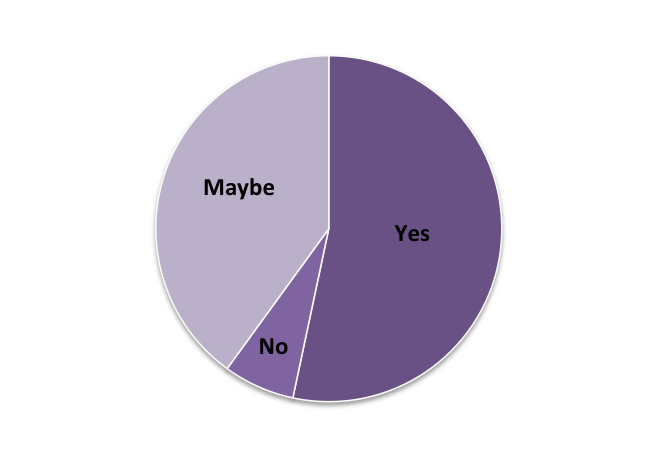
\includegraphics[width=0.35\textwidth]{figures/SurveyFig5rev}%
    \end{tabular}
    \qquad
    \rowcolors{1}{}{lightgray}
    \begin{tabular}{@{}lc@{}}
    \toprule
    Answer & Count \\
    \midrule
    Yes & 24 \\
    No & 3 \\
    Maybe & 18 \\
    Total & 45 \\
    \bottomrule
    \end{tabular}
    \caption{Responses to ``Would you be interested in joining a professional
    society focused around the topics of WSSSPE?''}
    \label{fig:SFig5}
\end{figure}

% \begin{table}[h!]
% \centering
% \caption{A WSSSPE society?}
% \label{tab:survey_society}
% \begin{tabular}{|l|c|}
% \hline
% {\bf Answer} &
% {\bf Count} \\ \hline
% Yes &
% 24 \\
% No &
% 3 \\
% Maybe &
% 18 \\
% Total &
% 45 \\
% \hline
% \end{tabular}
% \end{table}
%
% \begin{figure}[h]
% 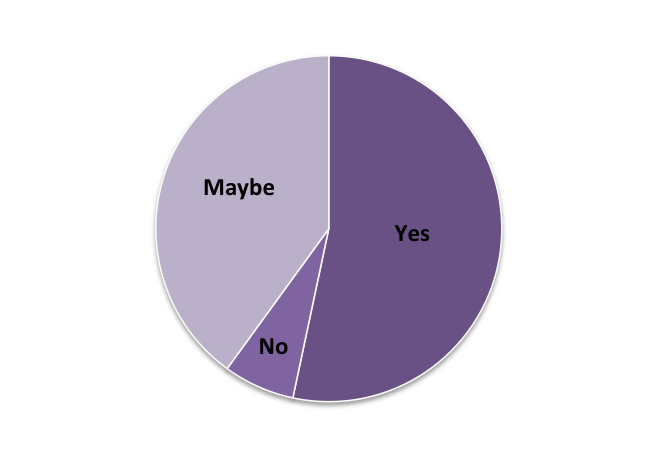
\includegraphics[width=0.4\textwidth]{figures/SurveyFig5rev}
% \caption{Would you be interested in joining a professional society focused around the topics of WSSSPE?
% \label{fig:SFig5}}
% \end{figure}


\newpage
\noindent \textbf{7. Will you be part of a working group  with colleagues going forward  on a topic addressed at WSSSPE, and if so, which one?}

\begin{figure}[h!]
    \centering
    \begin{tabular}{@{}c@{}}
        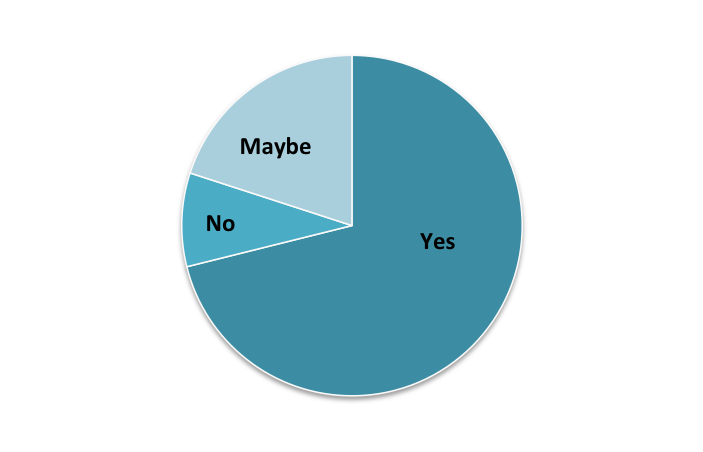
\includegraphics[width=0.35\textwidth]{figures/SurveyFig6rev}%
    \end{tabular}
    \qquad
    \rowcolors{1}{}{lightgray}
    \begin{tabular}{@{}lc@{}}
    \toprule
    Answer & Count \\
    \midrule
    Yes & 32 \\
    No & 4 \\
    Maybe & 9 \\
    Total & 45 \\
    \bottomrule
    \end{tabular}
    \caption{Responses to ``Will you be part of a working group  with colleagues
    going forward  on a topic addressed at WSSSPE?''}
    \label{fig:SFig6}
\end{figure}

% \begin{table}[h!]
% \centering
% \caption{Continuing working groups?}
% \label{tab:survey_continuing_wgs}
% \begin{tabular}{@{}ll@{}}
% \toprule
% Answer & Count \\
% \midrule
% Yes & 32 \\
% No & 4 \\
% Maybe & 9 \\
% Total & 45 \\
% \bottomrule
% \end{tabular}
% \end{table}

% \begin{figure}[h]
% 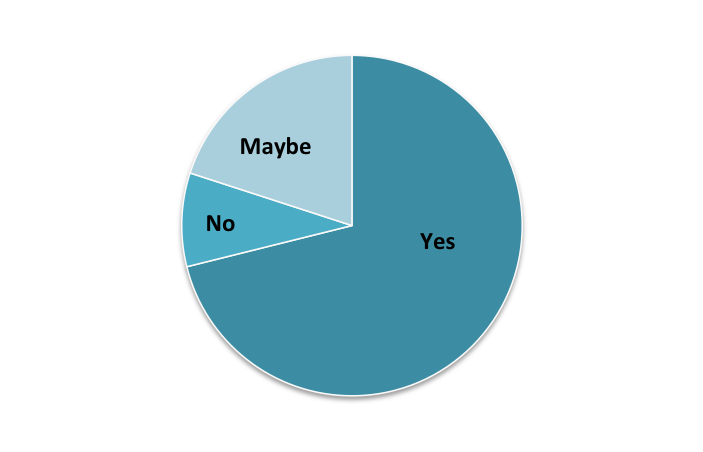
\includegraphics[width=0.4\textwidth]{figures/SurveyFig6rev}
% \caption{Will you be part of a working group  with colleagues going forward  on a topic addressed at WSSSPE?
% \label{fig:SFig6}}
% \end{figure}


\noindent \textbf{8. Working Group Name}

\vspace{0.2cm}

\begin{itemize}
\item ``Citations / CodeMeta''  and  ``Software Practices White Paper''
\item Best Practices White Paper and Best Practices Undergraduate Course
\item CodeMeta
\item CodeMeta
\item CodeMeta
\item CodeMeta, but I also supplied information to other working groups -- mostly connections to others -- that I hope will be of assistance.
\item Continuous CI for research software on uncommon hardware
\item Continuous Integration
\item Continuous integration for research software; Testing of scientific software
\item Curriculum for an undergraduate course on software best practices for domain scientists
\item Domain Specific Undergraduate Courses on Best Practices for Software Development
\item Domain Specific Undergraduate Courses on Best Practices for Software Development AND International Collaborations between institutions.
\item integration of software testing through Debian
\item Meaningful Metrics for Scientific Software
\item Meaningful Metrics in Software
\item metadata
\item multiple
\item Open Research Index, Metrics, Social Science, and maybe others
\item Prototypes
\item research software studies
\item Scientific Software Prototyping Infrastructure (S2PI), WG-Best-Practices
\item Setting up Software Sustainability Alliance
\item Software Sustainability Alliance
\item Software Sustainability Alliance; Metrics; White Paper
\item sustainability metrics; best practices
\item Sustainable Software Alliance
\item Sustainable Software Alliance
\item Tenure Letters
\item Testing in Sciences
\item Testing in Scientific Software
\item Verify Best Practices and Metrics for Sustainable Software
\item Verify Best Practices Case Studies
\item White Paper WG, Open Research Index WG
\end{itemize}

\noindent \textbf{9. Do you have any other comments or suggestions or ideas?}

\begin{itemize}
\item As a student, coming to WSSSPE4 has been very rewarding experience. Sustainable software is not my particularly sub-field of interest, but it was very interesting to me to apply the skills I had learned in my research in a different field. It definitely taught me a different perspective and expanded my original perception of where my skills can be applied.
\item As a student, this has helped me explore the different computational research careers and has made me more aware of scientific software best practices.  I found the plenary talks particularly valuable for learning about different areas of study, and it was great how willing all of the WSSSPE participants were to share more and help each other. I also found it valuable that there were other undergraduates at this WSSSPE, and it created another small community and encouraged me to participate more.
\item buddy me-sheet and workshop planning and moderation was excellent
\item Don't start at 8.45am if you're asking people to socialize and connect in the evenings! Work on getting a better gender, geographical and discipline balance. The use of travel bursaries has helped (particularly in getting early career participants).
\item Great organization, enjoyed being here very much, it was surely a success!
\item Great to meet colleagues from the UK and Germany at this event and enjoyed this format for working, engaging, and producing with the community while at the workshop that was facilitated by KnowInnovation.
\item I enjoyed the brainstorming session on Tuesday morning - well organized
\item I had hoped to have some discussion of building the sustainable communities beyond the software writing stage. The HPC focus, though expected slightly, was too heavy and I think ignores some of the other long term issues, such as preservation and addressing first principles for new technologies, or smaller, individual projects that will also support science. Perhaps it would be good to have a student session as well? (But I do like the integration).
\item I think the mixing of students, staff, faculty etc in the working groups is very effective and will contribute to  outcomes outside of the working group. It was great to see that we have undergraduates leading working groups here. There should be more attention on diversity.
\item I wish there were a project on training interns to work at academic environment as programmers
\item I would like to thank the committee for selecting me. As an undergraduate student this was a great experience I got to meet professors from the universities which I wanted to join. Now I exactly know how to prepare my application. I learned some really good technical skills and will definitely apply it to my research. So happy to be a part of this wonderful group. I will design a  logo for WSSSPE next year. Hope I can attend this event next year also.
\item Is there something better than sharpies (few of running around the room with a permanent marker)? Travel Awardee: Discussions here will and have benefitted my organization and community.
\item It was great to connect with people doing research software engineering in various positions, contexts, and universities. I felt like I learned a lot. Moving between the two rooms was a bit confusing.
\item Maybe involve more researchers from low-income countries if funds are available.
\item no. I think the moderator and the format are both great.
\item Nothing comes to mind
\item Receiving a travel award was crucial for me to come to WSSSPE4 this time, especially because WSSSPE4 was held outside the US. On the other hand, I see the great benefit this had on the geographic diversity of the participants, so I do think that meetings not only in the US are of great value. And again, I would like to emphasize, that travel awards are crucial for this type of meeting, as most participants are not directly supported for this type of activity - one reason to have a WSSSP5. (on another note: have a multi-line text field for comments next time)
\item The issue of software sustainability is on par with the challenges of building scientific instruments. Part of what I am for my doctoral dissertation is finding better abstractions, which leads to sustainability through better mathematics. This workshop raised my awareness in several other aspects, which will be considered for this and all future projects I may be related to.
\item The travel award made it possible for me to come to WSSSPE-4 and broaden my horizons.  Many issues pertaining research software and sustainable software were uncovered, and WSSSPE-4 brought to light the importance of the issues.  I'd encourage other travel awards to people, like me, who do not belong to the community.
\item There aren't lots of researchers knowing such kind of concept, sustainable software. We need to let more RSE know it.
\item There is a lot of discussion, but it's hard to see what actually will come of it. The discussion of the 9 working groups from last year at the beginning of the workshop clearly showed this: IIRC, not one had produced anything, all seemed to be stalled somewhere. We ought to find ways to actually make things *happen* after we talk about it (and admittedly have many good ideas).
\item This has been my first WSSSPE, and as someone coming from the humanities with an interest in RSE it has been an enormously rewarding experience to be able to interact with and learn from individuals and initiatives that have been part of the greater discussion around WSSSPE topics more in both quantity and quality. For me personally, it made me aware that I really need to refactor a lot of my basic assumptions for a PhD thesis, but that's a great thing because it means that I was able to draw on the exchanges and experiences from WSSSPE already. All in all, the workshop has made me more determined to become more involved with this community. And last but not least i just wanna say THANK YOU for the generous travel support I've received, which meant that my PI and dept. didn't have to have any doubts whether I'd drain their resources which are meant to be used towards achieving a completely different research goal.
\item This was an excellent mix of people, timed/structured activities, and untimed events.
\item This was an excellent mix of people, timed/structured activities, and untimed events. I had the opportunity to talk to numerous people about projects, issues, and ways to improve science/scientific software, and leave with many new ideas and possible collaborations/cooperative efforts with complementary projects. The working groups activities were excellent, a good mix of projects, and I saw a lot of progress on several I'm very interested in. (Please group this survey with my earlier one; I hit ``end'' too soon on the other! Thanks!)
\item We have activity on slack, github, and twitter. And working groups have their own stuff. Can we index these in a single place?
\item What percentage of the working groups actually end up producing anything? It seems to me as though most come up with an idea and then find out they don't have the resources to implement it - nice as the ideas are. Also, I assume someone is going to attempt to reinvent metrics or best practices every single year, I guess that's unavoidable.
\item WSSPE seems to be evolving nicely from year to year.  I hope that in WSSSPE5 there are lots of results to report from the outcome of WSSSPE4 working groups.
\item You could try unconferences instead of tracks.
\end{itemize}
